\documentclass{article}
\usepackage[a4paper,bottom = 0.65in,left = 0.75in,right = 0.75in,top = 0.65in]{geometry}
\usepackage{graphicx}
\usepackage[inline]{enumitem}
\usepackage{amsmath}
\usepackage{array}
\usepackage{enumitem}
\usepackage[super]{nth}
\usepackage{wrapfig}
\usepackage{titlesec}
\usepackage[colorlinks=false]{hyperref}

\newcommand{\xfilll}[2][1ex]{
\dimen0=#2\advance\dimen0 by #1
\leaders\hrule height \dimen0 depth -#1\hfill}
\titleformat{\section}{\large\scshape\raggedright}{}{0em}{}
\renewcommand\labelitemi{\raisebox{0.4ex}{\tiny$\bullet$}}
\renewcommand{\labelitemii}{$\cdot$}
\pagenumbering{gobble}
%\newgeometry{top=0.45in,left=0.75in,right=0.75in,bottom=0.45in}

\begin{document}
{\textbf{Email-id : sagar1singh109@gmail.com \hfill{ Contact : +917400401280}
\vspace{-5pt}
\begin{flushright}{Homepage : \url{http://homepages.iitb.ac.in/~170100115}}\end{flushright}}}
\vspace{-5pt}
\hspace{-0.6cm}
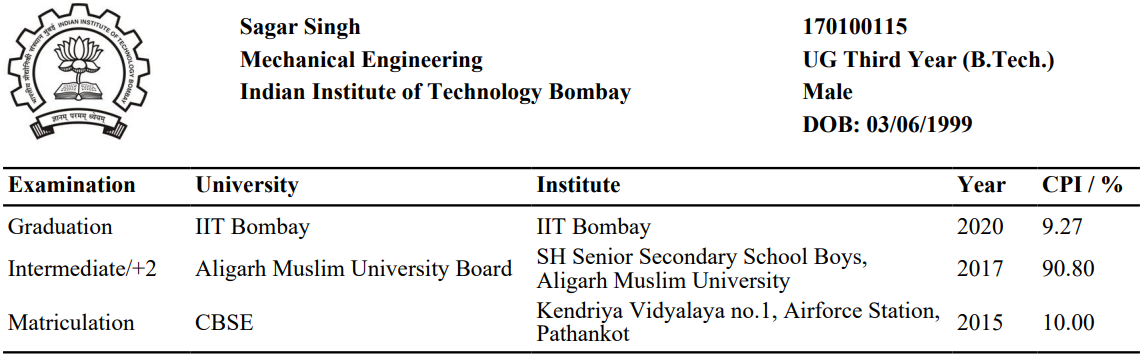
\includegraphics[width=\textwidth]{pic.png}
\vspace{-25pt}
%Proper acads begin 
\section*{{\LARGE Scholastic Achievements}\xfilll[0pt]{0.5pt}}
\vspace{-7pt}
\begin{itemize}[itemsep = -0.75 mm, leftmargin=*]
\item Currently \textbf{ranked in top 10\%} in a batch of \textbf{150 students} of Mechanical Engineering Department \hfill{\sl \small ('19)}
\item Ranked in \textbf{top 0.1\%} in Joint Entrance Exam (JEE) Mains among \textbf{12,00,000} students \hfill{\sl \small ('17)}
\item  Amongst top \textbf{1\%} in Joint Entrance Exam (JEE) Advanced among \textbf{2,20,000} students \hfill{\sl \small ('17)}
\item Ranked \textbf{\nth{10}} in Aligarh Muslim University Engineering entrance exam among \textbf{22,000} students\hfill{\sl \small ('17)}
\item Secured \textbf{national rank of 86} in National level Science Talent Search Examination \hfill{\sl \small ('16)}
\item Qualified \textbf{National Defence Academy (NDA)} entrance exam among \textbf{6,00,000} students \hfill{\sl \small ('17)}
\item Recipient of UP Science Talent \textbf{scholarship} for clearing \textbf{UPST Exam } \hfill{\sl \small ('17)}\\
% \item Secured state rank of 24 in Punjab in National Science Olympiad \hfill{\sl \small ('14)}
\vspace{-15pt}
\end{itemize}
%Proper acads end
%Start of the Academic Projects 
\section*{\LARGE Key Projects \xfilll[0pt]{0.5pt}}
\vspace{-5pt}
\textbf{\large{IIT Bombay Racing team}} \hfill{\sl \small (Feb'18-present)}
\vspace{-3pt}
 \sl \small Faculty Advisor- Prof. Amber Shrivastava, Dept. of Mechanical Engineering, IIT Bombay
\vspace{-2pt}
 Cross functional team of engineers who build an electric race car for Formula Student
International Competition conducted by SAE \& \textbf{IMechE} held at Silverstone, United Kingdom. We finished \textbf{\nth{4}} among electric teams
\textbf{\underline{Design Engineer \textbar \hspace{0} Drivetrain- }}} %Responsible for power transmission from motor to the wheels 
\begin{itemize}[itemsep = -0.75 mm, leftmargin=*]
\vspace{-3pt}
\item{Conceptualized \textbf{design, analysis and fabrication} of Drivetrain subsystem for the Season 2019-20 }
\item Carried out \textbf{efficiency analysis} of the motor by developing a \textbf{MATLAB} model to reduce \textbf{energy} consumption
\item Performed \textbf{Thermal analysis} of Gearbox in \textbf {ANSYS (fluent)} and analysed the \textbf{gears} in \textbf{KISSsoft}
\item Working on \textbf{Four-Wheel} drive by integrating \textbf{Compound} planetary gearbox and \textbf{In-Hub Wheel Assembly} 
\item Researched on alloys of \textbf{Titanium}, \textbf{Magnesium} and \textbf{Aluminium} along with \textbf{Aero \& High grade steels}
\item \textbf{Integrated} Planetary Gearbox and Tripod joint resulting in \textbf{25\% weight reduction} and better performance
\item Used \textbf{Optimum Lap} and \textbf{Simulink model} to simulate the total \textbf{time} taken for completion of race
 %to ensure that the inside working temperature range of gearbox is within the specified limits of Lubricating oil specifications

%\item Guiding trainees about the process of manufacturing, testing and designing of the components of Drivetrain
\vspace{-2pt}
\end{itemize}
 \textbf{\underline{Junior Design Engineer and Trainee-}}
\begin{itemize}[itemsep = -0.75 mm, leftmargin=*]
\vspace{-3pt}
\item Developed a \textbf{Bicycle model} to analyze the characteristic behaviour of a car for varying inputs
\item Performed \textbf{Topology Optimisation} on a experimental mount to reduce weight and remove excess material
\item Actively participated in \textbf{Vacuum Resin} infusion of carbon fibre to fabricate battery box and aero wings
%\item Actively participated and learned about the \textbf{vacuum resin infusion of carbon fibre} to fabricate battery box, aerodynamic wings and prototypes for testing
\item Analysed different \textbf{electric motors} best suited for upgrading to Four Wheel drive depending on their characteristics and compatibility by developing a model for \textbf{ideal motor curve} in \textbf{Simulink}
\item Worked extensively in various subsytems like Wheel assembly, \textbf{Vehicle dynamics} and Drivetrain
%\item Gained experience of the \textbf{practical} applications and relative \textbf{cost} of different \textbf{manufacturing techniques} and processes like Water-jet, Laser-cut, Welding, CNC, 3D printing, EDM, Anodizing and Hardening
%\item Manufactured \& designed motor controller mounts and driveshafts in \textbf{Solidworks} and analysed them in ANSYS 
\end{itemize} \\
\textbf{\large{Electrochemical Machining (ECM) of Micro Array Tool }}\hfill{\sl \small (Winter'19)}
\vspace{-3pt} 
{\sl\small Guide: Prof. Pradeep Dixit, Department of Mechanical engineering, IIT Bombay}
\vspace{-6pt}
\begin{itemize}[itemsep = -0.75 mm, leftmargin=*]
\item Investigated the effect of non uniform dissolution rate of 3*3 multi-tip micro tool array by ECM
%\item Carried out ECM simulations using COMSOL Multiphysics and validated the results by performing experiments 
\item \textbf{Modelled and Simulated} the process setup of ECM using \textbf{COMSOL} Multiphysics
\item \textbf{Validated} the above simulated results by the actual data obtained after carrying out \textbf{experiments}
\end{itemize}
\textbf{\large{Autonomous Aiming Bot} \textbar \hspace{} Institute Technical Summer Project} \hfill{\sl \small (May'18-Jul'18)}
\vspace{-4pt}
\begin{itemize}[itemsep = -0.75 mm, leftmargin=*]
\item  Built a \textbf{mobile} and \textbf{wireless} robot which uses \textbf{Raspberry pi camera} to obtain \textbf{live video-feedback} from distant locations to aim at a selected target precisely, it can be used to \textbf{automate shooting} purposes.
\item Provided \textbf{Two degrees of freedom} to the aiming mechanism by using step motors and microcontroller
%\item Achieved Wireless connection by establishing \textbf{SSH connection} with Raspberry Pi 
\item Fabricated the bot with \textbf{automatic operation} mode along with \textbf{manual mode} for better control
\end{itemize} 


\section*{\LARGE Other Projects and Technical activities\xfilll[0pt]{0.5pt}}
\vspace{-5pt}
\begin{itemize}[itemsep=-.25mm, leftmargin=*]

\item \textbf{Micro-Piezoresistive Accelerometer \& Pressure Sensor  }\hfill{\sl \small (Autumn’19)}\\
{\sl \small  [Guide: Prof. Pradeep Dixit, Mechanical Dept, IIT Bombay \textbar \hspace{0pt} Course Project]} 
\vspace{1.5pt}\\
-Simulated \& analysed MEMS (Micro Electro-Mechanical System) based piezoresistive sensors using COMSOL \\
-Proposed a fabrication and packaging method and validated simulated results with theoritical analysis

\item \textbf{Electrochemical Discharge based Micro Milling using Pulsed current }{\sl \small \hfill{\sl \small (Autumn’19)}}\\ 
{\sl \small  [Guide: Prof. Pradeep Dixit, Mechanical Dept, IIT Bombay \textbar \hspace{0pt} Course Project]} 
\vspace{1.5pt}\\
-Investigated the effect of Interelectrode Gap and Feed rate on the ECDM process of Micro channel formation by performing experiments and analysed the results 

\item \textbf{Helical Springs}{\sl \small  \hfill{\sl \small (Spring’19)}}\\
{\sl \small  [Guide: Prof. Parag Tandaiya, Mechanical Dept, IIT Bombay \textbar \hspace{0pt} Course Project]} 
\vspace{1.5pt}\\
-Carried out  \textbf{self designed} experiment of testing helical springs and their combinations under uniaxial tension\\
-Performed \textbf{Finite Element Analysis} to compare the experimental and theoritical results with the simulation 

\textbf{Automobiles \textbar \hspace{0} Summer of Science  } \hfill{\sl \small (May’18-Jul’18)}
\vspace{1.5pt}\\
-Completed areporton the mechanical response of a car by studying its systems and their interdependence
-Learned about the influence of important vehicle dynamics parameters on the performance of automobiles

\item \textbf{Jindal Steel Works (JSW) Dolvi - Industrial Visit  } \hfill{\sl \small (Oct'18)}
\vspace{1.5pt}\\
-Visited the 5 MTPA capacity plant and explored the processes of Blasting, Casting and Rolling \\
-Presented a report regarding various steps and regulations involved in Steel Making at Industrial level

\item \textbf{Autocar Performance Show 2018} \hfill{\sl \small (Dec'18)} 
\vspace{1.5pt}\\
-Attended India's largest car and bike Exhibition as a representative of IIT Bombay racing car

\item \textbf{Inter IIT Tech Meet} \hfill{\sl \small (Dec'18)}
\vspace{1.5pt}\\
-Coordinated with a team of 26 members from various disciplines to manage 760+ participants from all IITs

\item{\textbf{Robot building competitions} \hfill{\sl \small (Sep'17,'18)}}
\vspace{1.5pt}\\
-Built a Bluetooth controlled obstacle manoeuvring bot and a year later
mentored a team of 4 undergraduate \\  
freshers to make the same for institute level competition %\hfill{\sl\small(Aug'18-Sep'18)} 
\vspace{-5pt}
\end{itemize}

\section*{\LARGE Technical Skills \xfilll[0pt]{0.5pt}}
\vspace{-7pt}
\begin{tabular}{p{5cm} p{12cm}}
\textbf{Softwares}  & MATLAB, Simulink, SolidWorks, AutoCAD, Scilab, Optimum Lap \\
\textbf{Analysis tools} &  ANSYS (Fluent, Thermal, Structural), COMSOL,MSC-Adams, KISSsoft \\
\textbf{Programming} & C++, Python, HTML, Julia, CSS, JavaScript \\
\textbf{Electronics} & Raspberrry Pi, Common sensors/actuators, Micro-controllers, Arduino \\
\textbf{Others} & \LaTeX, G and M code, Linux (Ubuntu)
\end{tabular}
\vspace{-3pt}
\vspace{-7pt} %% had to put vspace two times, first one doesn't work
\section*{\LARGE Positions of Responsibility\xfilll[0pt]{0.5pt}}
\vspace{-7pt}

\textbf{Teaching Assistant \textbar \hspace{} Department of Civil Engineering} \hfill{\sl \small (Autumn'19)}\\
{\sl \small CE 102  \textbar \hspace{}  Engineering Mechanics under Prof. Amber Jain	}\\

\textbf{Teaching Assistant \textbar \hspace{} Department of Chemistry} \hfill{\sl \small (Autumn'19)}\\
{\sl \small CH 107  \textbar \hspace{}  Physical Chemistry under Prof. Amber Jain	}\\
\vspace{-17pt}
\begin{itemize}[itemsep = -0.75 mm, leftmargin=*]
\item Among the f undergrads selected as Teaching Assistant across all branches to mentor \& assist 250+ students
%\item Helped in providing quality accommodation to 5000+ participants and visitors
\end{itemize}\\
\textbf{Mentor \textbar \hspace{} IIT Bombay Racing Summer Induction Program}
\hfill{\sl \small (Feb'19 - Present)}\\
\vspace{-17pt}
\begin{itemize}[itemsep = -0.75 mm, leftmargin=*]
%\item \textbf{Framed} questions and coordinated with other subsystem heads for conducting \textbf{recruitment} test of the team %200+ students registered
\item Guided \textbf{8 trainees} to excel in the basics of race car engineering through literature study, simulations and tasks
\end{itemize}
\textbf {Mentor \textbar \hspace{} Summer of Science}
\hfill{\sl \small (May'19-July'19) } \\
\vspace{-17pt}
\begin{itemize}[itemsep = -0.75 mm, leftmargin=*]
\item Guided student about mechanical linkages, Simulations, CADs and assisted him in the completion of his report
\vspace{-14pt}
\end{itemize}
\textbf{Co-ordinator \textbar \hspace{} Hospitality \textbar \hspace{} Mood Indigo 2018} \hfill{\sl \small (Sep'18 - Dec'18)}\\
{\sl \small Asia's largest college cultural festival $|$ Footfall: 141,000+ $|$ 210+ events $|$ 160+ international artists $|$ 30+ venues}\\
\vspace{-17pt}
\begin{itemize}[itemsep = -0.75 mm, leftmargin=*]
\item Worked in a team of 30 members, managing the hospitality needs of \textbf{1.4 lakh+} visitors
%\item \textbf{Managed} with college representatives all across the country to publicize events \& competitions of Mood indigo
%\item Helped in providing quality accommodation to 5000+ participants and visitors
\end{itemize}
% \textbf{Organiser \textbar \hspace{} Inter IIT Tech Meet 2018}
% \hfill{\sl \small (Sep'17 - Dec'17)}\\
% \vspace{-17pt}
% \begin{itemize}[itemsep = -0.75 mm, leftmargin=*]
% \item Coordinated with a team of 26 members from various disciplines to manage 760+ participants from all IITs
%\item Helped in the organisation of the event-Engineers Conclave in which 20+ IITs demonstrated their top projects
% \vspace{-3pt}
% \end{itemize}
\section*{\LARGE Courses Undertaken\xfilll[0pt]{0.5pt}}
\vspace{-7pt}
\begin{tabular}{p{4cm} p{12.5cm}}
\textbf{Mechanical courses} & \vspace{-7pt} Fluid Mechanics$ ^+ $, Computational Fluid Dynamics and Heat Transfer, Thermodynamics, Heat transfer$ ^+ $*, Engineering Metallurgy, Manufacturing Processes$ ^+ $, Mechanical Measurements$ ^+ $, Strength of materials, Solid Mechanics$ ^+ $ Engineering Mechanics, Engineering Graphics \& Drawing$ ^+ $, Design for Manufacturing, Micro Electro Mechanical Systems \\
\textbf{Systems and control} & Mathematical Structures for Systems and Control, Microprocessors and Automatic Control$ ^+ $*, Kinematics and Dynamics of Machines$ ^+ $* \\
\textbf{Mathematics} & Calculus, Linear Algebra, Differential Equations, Numerical Analysis\\
\textbf{Chemistry} & Organic Chemistry, Physical Chemistry$ ^+ $, Inorganic Chemistry$ ^+ $\\
\textbf{Physics} & Quantum physics and applications, Basics of electricity and Magnetism$ ^+ $\\
\textbf{Others} &  Industrial Engineering and Operations Research, Operations Management, Electrical \& Electronics Circuits, Biology, Economics*, Computer programming and Utilization$ ^+ $, Psychology, Environmental Studies \\
\end{tabular}
\vspace{-8pt}
\item{\hfill{\sl \small Courses with * to be completed by summer' 20}} 
\vspace{-5pt}
\item{\hfill{\sl \small Courses with $ ^+ $ are accompanied by lab}
}
%End of POR's
%Extra cirricular
%Courses start
\vspace{-16pt}

\section*{\LARGE Extracurriculars\xfilll[0pt]{0.5pt}}
\vspace{-5pt}
%\textbf{Sports and Culturals}
%\vspace{-5pt}
\begin{itemize}[itemsep=-.75mm, leftmargin=*]
%\item Successfully completed a two month basic course of \textbf{German Language} under cult school \hfill{\sl \small ('17)}
\item Received \textbf{80 hours} of training and completed an intermediate level one year training in \textbf{Basketball} NSO \hfill{\sl \small ('18)}
\item Completed training and endurance test by continuously \textbf{swimming 1.55 Km} in \textbf{one hour} \hfill{\sl \small ('19)}%after taking Intermediate level of training in swimming learning freestyle, breastroke, backstroke and butterfly strokes.
\item Won \textbf{two} consecutive \textbf{gold} medals in inter school basketball competition at Aligarh Muslim University \hfill{\sl \small ('16,'17)}
\item Awarded \textbf{best Project} at Regional level National Children Science Congress \hfill{\sl \small ('14) }%on the theme Weather, Cl}imate, Society and Culture in Kendriya Vidyalaya Jammu region
\item Participated two times in Regional Sports meet in \textbf{Kho-Kho} at Kendriya Vidyalaya Jammu region \hfill{\sl \small ('12,'14)}
\item Won several medals in \textbf{Football} and \textbf{Kabaddi} at Kendriya Vidyalaya Airforce Station Pathankot \hfill{\sl \small ('13)}
\item Participated in Regional \textbf{Youth parliament} competition held at KV Army Area, Pathankot \hfill{\sl \small ('14)}
\\
\vspace{-3pt}
\end{itemize}






\end{document}